\documentclass[../main.tex]{subfiles}
\graphicspath{{subfix{../Images}}}

\begin{document}
    \subsection{Data Encryption}
        The solution proposed is based on publicizing data in a publicly accessible ledger. In order to achieve and maintain voter privacy, data published in this medium needs, at least, a layer of encryption needs to be applied to it before entering the public structure. This encryption must provide two functionalities: prevent other users from determining the voting options of a specific voter or voters, and prevent the calculation of the final tally before the intended process step.
        \par
        Asymmetrical encryption schemes are an obvious, simple and efficient solution for this problem. Our proposed system maintains three essential actors: voters, voting booth contracts, and the tally contract. Each actor can create a pair of asymmetrical keys and distribute the public key, but for our specific case, this task is limited to the smart contracts, i.e., voting both and tally. This removes some complexity from the voter perspective and deposits it into programable software scripts, which allows for an automation of this process. As such, each voting booth contract and the tally contract generate a pair of asymmetrical encryption keys, with the public key in each one provided to a voter alongside with the Vote NFT used to contain their election choices. 
        \par
        Section \ref{multiple_vote_casting} presents a more detailed exposition on how the encryption scheme is implemented in this protocol.
        

    \subsubsection{Data Obfuscation}
        Vote data is double encrypted with the tally contract key and the respective voting booth contract key, i.e, the public encryption key provided by the voting booth contract that mints the Vote NFT requested by a voter. A double encryption scheme using a pair of keys from a larger set increases the solution space for the resulting ciphertexts, which makes a statistical analysis of the encrypted votes harder, but not completely impossible. In any election, the universe of choices for a given question is finite. If no additional obfuscation methods are employed, especially if any encryption efforts are performed with a small number of encryption keys, the solution space for generated ciphertexts may be small enough to warrant the use of statistical tools that can provide relevant information about the final result before the end of the election.
        \par
        For example, consider an election that requires a voter to chose one of four choices: \textit{A, B, C, or D}, a simple encryption scheme that advances the selected option ten positions in the alphabet, and with only one encryption layer, it is easy to understand that the solution space is simply \textit{K, L, M, N}. Determining the final tally without decrypting the vote data becomes a trivial operation. Adding "salt", i.e., a piece of random data, to the plaintext before encrypting it solves this issue because it extends the solution space so that statistical analysis of the encrypted data becomes infeasible.
        \par
        The value of salt in itself is irrelevant since it gets discarded after decrypting the "salted" data. The difficulty of obtaining true random values in a blockchain, which is purely deterministic, is well known \cite{Antonopoulos2018}, but for our purpose, a pseudo-random number is sufficient since we are not using it to generate critical system information, such as encryption keys or other cryptographic element. Using portions of a hash digest is a popular option to obtain pseudo-random values in a simple and fast fashion. Popular hash functions, such as the ones in the \textit{keccak} family used in the Ethereum blockchain, can be applied to another pseudo-random piece of data, such as the current UNIX timestamp for example, to obtain these salt values.
        \par
        Salt values are appended to the vote information before encrypting it with the public key from the tally contract (inner encryption layer).

    \subsubsection{Private Key Management}
        The universe of key pairs is equal to the number of smart contracts used to support the election,which are all the voting booth smart contracts plus one, the tally one. The transparent nature of these contracts prevents any sensitive information from being published in their code, namely, writing the private keys in the corresponding contracts defeats the whole encryption effort since anyone can check the contract source code and decrypt data stored under it. We solve this problem by relying on the thrusted third party that we are already using to determine voter eligibility.

    \subsection{Multiple Vote-Casting}
        \label{multiple_vote_casting}
        Multiple vote-casting is a feature used to combat vote coercion by a coercer, here defined as someone that can influence how a voter casts his or her choice either through positive, (money offers, gifts, etc) or negative (blackmail, threats of violence, etc.) reinforcement, by allowing voters to cast multiple votes in an election and counting only a single one. Vote coercion is an undesirable behaviour for any voting system, electronic or not, since it defeats the basic purpose of the exercise. This approach was implemented in e-voting solutions such as the Estonian i-Voting system \cite{Madise2006}, the Norwegian e-Vote project \cite{Barrat2012}, and even TiVi, a blockchain-based e-voting solution \cite{TiVi2021}. In all the examples indicated, a voter can submit multiple votes electronically during the election window, and only the last one gets counted. The Estonian i-Voting system, which was deployed in Estonia's 2005 national elections in parallel with a traditional paper ballot system, prioritised the physical vote over any electronic one as well.
        \par
        The idea behind this approach is to remove incentives from coercers. Even if they are able to "convince" someone to vote against their will, voters always have the opportunity to replace the coerced vote later on or, in the Estonian case, vote physically if they are unable to do so freely from an electronic platform.
        \par
        We intend to implement a similar, NFT-adapted feature in our proposed solution. The increment in solution complexity is negligible since we already benefit from the fact that we operate with digitally unique NFTs as vote abstractors. In our approach we considered a strategy based on the replacement of submitted Vote NFTs, i.e., once submitted, the metadata of a Vote NFT cannot be altered, but a submitted token can be replaced by another cast at a later stage, as long as it happens within the voting window defined.
        \par
        To implement such feature, we need to ensure the storage strategy used allows for future replacements of submitted tokens while, simultaneously, ensuring voter and vote privacy, i.e., that any voter information, as well as their choices in the current election, are protected. To ensure privacy along the whole process, multiple layers of encryption are applied to the sensible data, namely, voter specific information and ballot choices. Data encryption is performed at the smart contract level, i.e., invoking contract functions. Public encryption keys for this purpose are shared within the contract code.
        \par
        Vote NFTs are stored at the contract level using an hash map, a popular storage strategy in distributed environments. The hash value used to index Vote NFTs is calculated before the submission of the Vote NFT, at the user level, where his or her personal information is available and can be prepared such that it produces a unique indexing hash. The usage of already unique identification numbers in this process, such as a National ID number, a Tax Revenue Service ID, Social Security Numbers, etc., ensures this outcome.
        \par
        The full process flow for this feature is represented in Fig. \ref{fig:multiple_vote_casting}.

        \begin{figure}[htp]
            \centering
            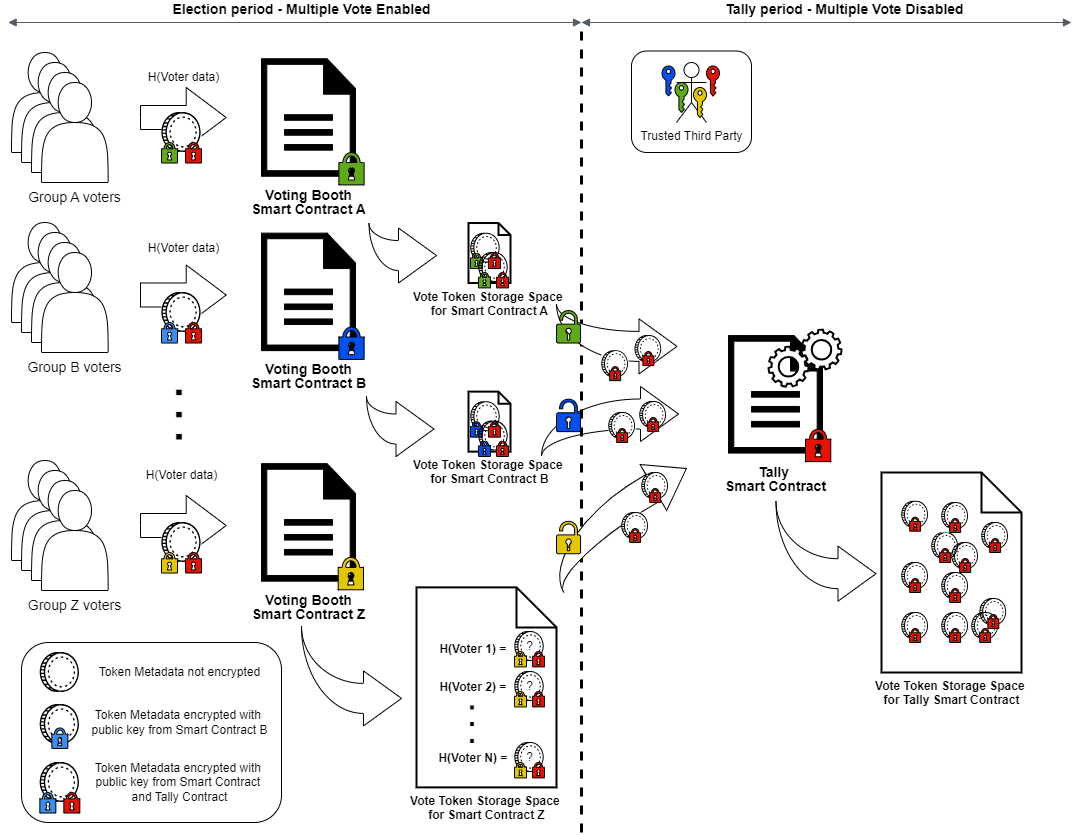
\includegraphics[width=0.8\textwidth]{../Images/MultipleVoteCastingLogic.png}
            \caption{Implementation logic to allow for multiple vote casting.}
            \label{fig:multiple_vote_casting}
        \end{figure}

        \par
        The submission of a Vote NFT also includes a hash digest that is unique for all voters and can be used to retrieve that Vote NFT cast previously by a voter without revealing its contents. During the election period, successfully submitted Vote NFTs are stored under the respective voting booth smart contract. The actual storage location for these tokens is dependent of the blockchain architecture considered but it is not critical for this explanation.
        \par
        Privacy is assured via double encryption of the vote data by a pair of keys supplied from the voting booth contract and tally contract. The private encryption keys required to decrypt all the voting data have to be securely stored during the whole exercise. A sensible and sensible approach is to entrust them to the same trusted third party that ensures the integrity of the list of eligible voters, but other options may be of consideration.
        \par
        During the election window, users can request and submit multiple Vote NFTs, each replacing any one previously submitted. Once this window terminates, the tenuous link between the tokens and their owners is broken upon sending them to the tally contract. This operation also removes the layer of encryption that could be used to divide the tokens per voting booth, thus achieving anonymity between the voters and their choices. Vote NFT tokens are stored under the tally contract under no specific order.
        \par
        The final tally is determined by removing the last layer of encryption from the tokens metadata and computing the final result. Another potential, more private approach, consists in computing the tally homomorphically and decrypt only the final result. This approach extends the privacy related to the contents of the actual votes, but given that all links to the voters who cast them are already removed, the gains with such approach are negligible considering the added complexity and resource consumption.

    \subsection{Security Analysis and Assessment of Threats}
        The security of e-voting systems has been the subject of academic research, and it has coalesced around the definition of security criteria, such as voter privacy, transparency, accuracy, etc. These criteria are met through the implementation of, typically, cryptographic features that increase the security of the system against dishonest actors. A simple example is using encryption to protect the information in a vote to achieve vote privacy. The number and type of criteria used for this characterization differ from publication to publication, but some attempts have been made over the years to normalise this exercise. In one of the latest publications dedicated to this effort, \cite{Almeida2023} presented a literature survey that established a series of five criteria deemed "minimal" as the base set from an analysis of a number of publications that employed such characterization to determine the security offered by the proposed solution.
        \par
        Alongside with this analysis, we also include an assessment of potential threats included in each criteria considered, namely, concrete attacks that have been employed on previous e-voting systems and how the proposed system is able to protect itself and/or nullify them. \cite{Zissi2011} includes a detailed list of potential threats affecting e-voting system without differentiating between any of the architectural paradigms considered. We adapted this list to our architecture and repeated the threat analysis from the reference point of a decentralised e-voting system. 
        \par
        The following analysis is going to focus on the following security criteria:
        \begin{enumerate}
            \item{Accuracy - A voting system is accurate if it does not allow for changes to a vote after submission, changes to the final tally, or invalid votes.}
            \item{Eligibility - Voting systems that allow only registered or valid voters to submit votes implement eligibility.}
            \item{Privacy - A private voting system is able to remove all the links between personal information related to the voter and the vote submitted.}
            \item{Verifiability - A voting system is considered verifiable if it allows for independent confirmation of the submission of a vote by the voter.}
            \item{Robustness - A robust voting system is able to prevent and even withstand the actions of dishonest voters to prevent the successful and accurate completion of the voting exercise.}
        \end{enumerate}

        The remainder of this section analyses the e-voting solution detailed in this proposal according to the framework for minimal security criteria presented in \cite{Almeida2023}.

        \subsubsection{Accuracy}
            Encoding votes into NFT metadata ensures that this information is written into the blockchain. In both approaches considered, once the NFT is written into a block and is part of the chain, the contents of a vote become immutable due to the computational infeasibility of modifying data on the chain.
            \par
            The final tally is the output from a smart contract function, which adds transparency to the process but does not negate the possibility of an erroneous result or detect any invalid votes. A smart contract function can be used to ensure the correct format of a vote before counting it. Assuming a deterministic computation of the final tally, this means that changes in it imply unauthorised changes to the number of Vote NFTs submitted. An expansion of the previous reasoning negates this scenario as well, since such a change to the number of votes submitted, as well as the number of Vote NFTs stored, implies adding and/or removing information from the blockchain, which we have already stated is computationally infeasible.
                
                \paragraph{Threat Assessment}
                The accuracy of an e-voting system can be affected by adversarial activities such as:
                \begin{itemize}
                    \item{Wiretapping}
                    \item{DNS attack}
                    \item{Malicious code on client}
                    \item{Hardware modification, substitution and interception}
                    \item{Software modification, deletion, edition, trojan horses, information leaks, trapdoors and viruses}
                \end{itemize}

                Basing our solution on a blockchain immediately nullifies many of the threats considered above. The immutable and transparent nature of blockchain make threats based on an adversary being able to alter the system's software and/or hardware irrelevant, as well as any threats from wiretapping communication channels. Software is deployed mainly as smart contracts, which prevents unwanted and undetectable changes to the code used for the core properties of the system. Blockchains also notoriously abstract most hardware characteristics from its overall workings, so, as long as nodes execute protocol code as intended, any hardware alterations do not pose a threat. 
                \par
                The most serious threat from this list is the existence of malicious code on a client. The core of the system runs on a distributed, public network, but the submission of individual votes requires an interface that is served from the client side. Realistically, an adversary can replace this interface with a different one without the user noticing it. The risk here is the loss of private information, such as private encryption keys and personal information. If an adversary is able to, for example, control the interface used by someone else to submit votes, such as controlling an unlocked and previously authenticated device (theft, blackmail, threats of violence, etc.), installing remote control software in a device without the owner's permission, etc., he or she can submit a vote under another person's identity. It is very hard to protect the system against such deep level of control. To counter this threat, we provide a multiple-vote casting feature, but in the end, it is the voter that needs to detect an erroneous submission from his or her platform, which is eased by providing voting receipts and an history of interactions with the smart contracts that process the submissions, and provide a replacement vote according to the voter's wishes, as well as reporting this attempt to the relevant authorities. As indicated above, the actions that an adversary has to undertake to be able to cast a vote as someone else can be considered criminal offenses with penalties foreseen in most legislative frameworks. 

        \subsubsection{Eligibility}
        \label{voter_eligibility}
            The sensible nature of elections prevents the full decentralisation of an e-voting system, at least regarding the presence of a trusted authority that determines the individual eligibility of each voter based on whatever rules exist to regulate a given election (e.g., age, nationality, professional status, etc.). Unless an election is free, i.e., without any regulations regarding who can vote, there is a requirement for a mechanism to implement limitations on the set of voters that are eligible to participate in it. For example, it makes sense to exclude teachers and other non-student school workers from an election used to select a representative from the student body.
            \par
            For our proposal, we consider two approaches to solving this problem in a decentralised fashion:
            \begin{itemize}
                \item{using a centralised database to store eligibility information and access it from the decentralised e-voting system using an oracle. Any oracle used for this effect replies to a query in boolean format, i.e., if a voter is (\textit{true})} or is not (\textit{false}) eligible to participate in the election based on the data returned from the centralised database.
                \item{using a cryptographic accumulator, used to prove membership. Instead of storing all the eligible voter data, it can be "accumulated" instead into a root value. We can use the accumulator's properties to infer if a given piece of data related to a specific voter is present in the root value or not, thus also obtaining a boolean reply in this regard, like with the previous method.}
            \end{itemize} 
            Another possible approach is the usage of SoulBound NFTs for identification purposes, a strategy used in \cite{Sagar2023}. But unfortunately, these NFTs are still in their infancy regarding their applicability in other areas, and this approach is omitted from the presented solution.
            Sections \ref{centralised_eligibility_database} and \ref{cryptographic_accumulators} provide additional details regarding the two approaches considered in determining voter eligibility in our solution.

            \paragraph{Oracle Accessible Centralised Eligibility Database}
            \label{centralised_eligibility_database}
                The basis of our eligibility problem derives from the limitations of current blockchain implementation in storing large quantities of data. Though it is technically possible to do so, storing even a small list of eligible voters directly on the chain is very inefficient, both from an economic (due to potential gas costs) and resource management perspective. This issue is actually pertinent across several application domains, and, as a consequence, several strategies to allow blockchain to access external data, i.e., off-chain data, have been proposed.
                \par
                \cite{Ezzat2022} presents an exhaustive study on these strategies, which are used to establish communication protocols to enable the exchange of data with external data sources or even other blockchains. Among these, oracles stand out as one of the most promising in terms of flexibility and ease of implementation. Blockchain oracles are implemented as smart contracts that use their functions to query data from the outside, namely by requesting it from an external source, similarly to a regular API. Due to this perception, oracles are often seen as "blockchain middleware," decreasing the gap between blockchains and the external world. A simple example of oracle use can be found in crypto exchange platforms that allow for trade between different cryptocurrencies. The value of each tradeable cryptocurrency is currently very volatile and often dependent on speculative factors. Since blockchains themselves do not store the exchange rate of their native token relative to a fiat currency, which is the parameter to consider in inter-blockchain trades, this information is kept instead in "traditional" centralised sources that maintain APIs that can be used to retrieve this information remotely. Oracles are often used in these cases to retrieve the exchange rate of the tokens involved (external information) and provide a fairer exchange of tokens (internal operation).
                \par
                Oracles fit quite well in our solution. Eligibility data is stored in a conventional, centralised database, and the eligibility state of a given voter is obtained by invoking a function in the smart contract that implements the oracle. Oracles are relatively easy to construct, but they do increase the centrality of the solution while potentially creating a point of failure in the system. External data sources are not subjected to the blockchain protocol and data redundancy that ensure its integrity, and thus can be corrupted with less effort. Therefore, using an oracle in this fashion also requires a trusted third party to ensure the integrity of the external data, which moves this solution away from a purely decentralised one.

            \paragraph{Cryptographic Accumulators}
            \label{cryptographic_accumulators}
                Cryptographic accumulators, also known as set accumulators, are cryptographic primitives that use unidirectional hash functions to represent a set of elements through an \textit{accumulator value}, a single and constant-size value that can be used to determine if a given element belongs to the set without revealing the set contents at any point of the verification process. A hash function $ y = H(x) $ is such that it receives an input $ x $ with arbitrary length to produce a fixed-sized output $ y $, also known as \textit{hash digest}. The unidirectionality of the hash function derives from the fact that:
                
                \begin{enumerate}
                    \item{For all $ x \in \{0, 1\}^* $ it is computationally easy to calculate $ y = H(x) $}.
                    \item{For all $ y \in \{0, 1\}^n $ it is computationally infeasible to find $ x \in \{0, 1\}^* $ such that $ H(x) = y $}.
                \end{enumerate}

                A desirable hash function is also one that provides collision resistance, i.e., it is computationally infeasible to find two input elements, $ x_1, x_2 \in \{0,1\}^* $, such that $ H(x_1) = H(x_2) $, which enables hash digests to be used as data fingerprints, a strategy commonly used to ensure data integrity during communications, software certification during distribution, etc. Among the various use cases of cryptographic accumulators, we highlight \textit{anonymity enhancement} and \textit{identity management} as the most pertinent for our case. Set accumulators can be static or dynamic, depending on their ability to add and remove elements from the original set without requiring the re-calculation of the \textit{cumulative set} \cite{Loporchio2023}. For our particular context, static accumulators are preferable. By publishing the \textit{cumulative value} of the set of eligible voters using a static accumulator, this means that the list of eligible voters "is closed," meaning that, for better or worse, no voters can be added or removed after this publication without changing the \textit{cumulative value} published. 
                \par
                \cite{Benaloh1993} introduced set accumulators as, in a simplistic fashion, the hash digest of the cumulative value of the hash digests of the elements of the set. To determine the \textit{cumulative value} of a set accumulator, one begins by determining the hash digest of every individual element. From there, hash digest pairs are concatenated and re-hashed to obtain a digest of the hashed pair. This process continues until one value remains: the \textit{cumulative value}. Fig. \ref{fig:accumulator_example} illustrates this process.

                \begin{figure}[htp]
                    \centering
                    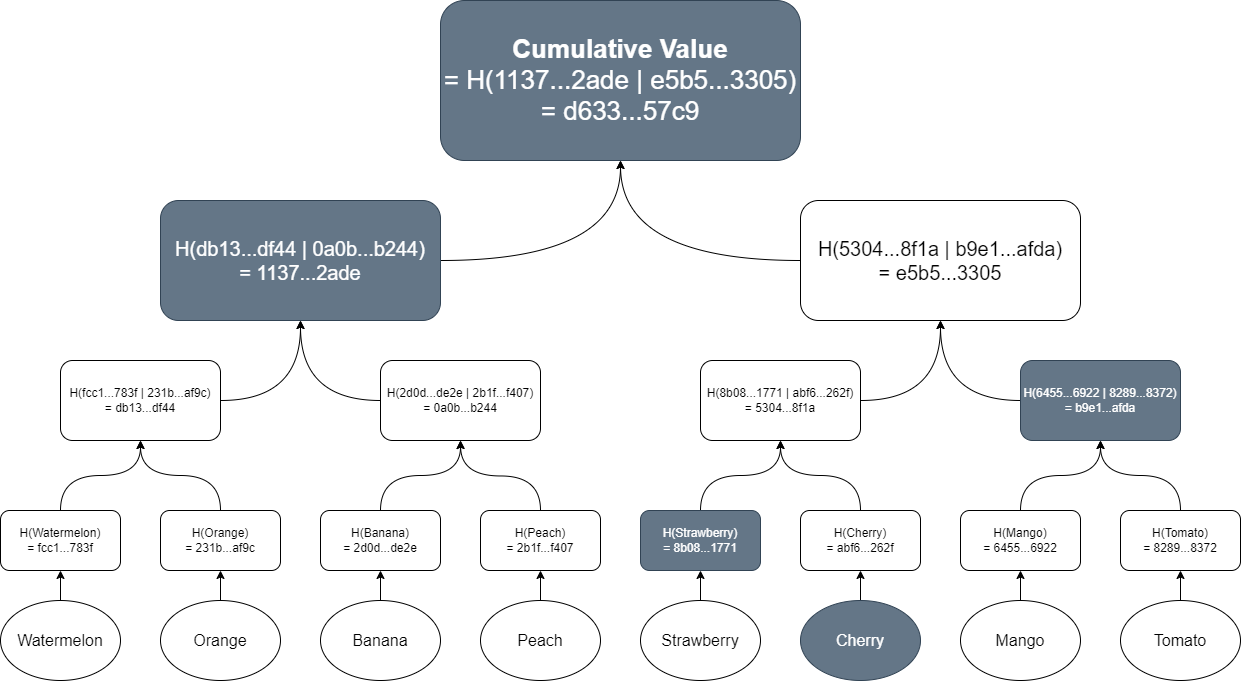
\includegraphics[width=0.8\textwidth]{../Images/AccumulatorExample.png}
                    \caption{Simple example of an accumulator to represent a set of strings.}
                    \label{fig:accumulator_example}
                \end{figure}
                
                An independent verifier can verify the membership of an element by obtaining a minimum of partial results and recalculating the \textit{cumulative value}, starting with the element whose membership he or she desires to verify and combining the successive hashes with the ones provided. If the \textit{cumulative value} obtained matches the one published, the unidirectionality and collision resistance of the hash function used guarantee, with reasonable certainty, that the element does belong to the original set. Taking the example presented in Fig. \ref{fig:accumulator_example} into consideration, if an independent verifier wishes to determine if "Cherry" belongs to the original set, he/she only requires knowledge of the \textit{cumulative value} and the partial calculations indicated in grey in the figure. From there, the verifier can use the hash function used to determine this value to re-calculate the \textit{cumulative} one without requiring any knowledge about the remaining elements of the original set or needing to re-hash every element. Providing only the intermediary hashes to the independent verifier allows for the remaining set elements to remain secret since it is computationally impossible to determine which strings originated from the hash digests provided.
                \par
                Cryptographic accumulators present a solution that benefits from the advantages of storing relevant data directly in the blockchain while keeping that data to a minimum of the required storage space \cite{Wang2021a}. This approach is not novel: in \cite{Chen2020}, the authors use accumulators to optimise a UTXO (\textit{Unspent Transaction Output})-based blockchain by storing the \textit{accumulated value} of the UTXO set in the blockchain instead of the whole set. \cite{Wang2022} apply cryptographic accumulators to authenticate users in an \textit{IoT (Internet Of Things)}-based blockchain, similarly to our proposed strategy.
                \par
                Our approach is to use a set accumulator to obtain the \textit{cumulative value} of all eligible voters, and then use membership functions to determine if a given voter is eligible for the exercise based on the output from the membership function. This eliminates the need to access external data sources while keeping the additional data stored in the chain to a minimum.

                \paragraph{Threat Assessment}
                \begin{itemize}
                    \item{Impersonation}
                    \item{Falsification of messages}
                    \item{Spoofing}
                    \item{Man-in-the-middle Replay attacks}
                \end{itemize}

        \subsubsection{Privacy}
        \label{voter_privacy}
            The way voter privacy is achieved in our system depends on the approach considered, given how important the storage mechanism is to the criteria. But both approaches are able to achieve it.
            \par
            In a contract-based approach, the link between Vote NFT data and the entity that created it is maintained solely in the data structure that maps a specific, unique Vote NFT to an address. The privacy of a voter depends on how hard it is to determine the identity behind these addresses, which is an issue transversal to all blockchains. It is possible to use statistical tools that analyse blockchain transactions to increase the probability of discovering who is controlling an address, but these often rely on the existence of a significant number of transactions with that address. If a voter uses a specific address solely for voting purposes, this threat diminishes greatly. Additionally, in this approach, vote metadata is always encrypted when the NFT gets stored in the contract. So even if the identity of the voter behind an address gets revealed somehow, the adversary would still have to decrypt the metadata somehow to have any impact on the voting exercise. The pseudo-anonymity of blockchain operations plus the added layer of encryption to the sensible data ensure voter privacy in this system.
            \par
            Account-based blockchains simplify this feature by assigning private storage domains that ensure that any sensitive operations, namely the voting act itself, occur in a personal space protected cryptographically. To gain access to such space, an adversary needs to discover the private counterpart of the asymmetrical encryption key pair used to set up the account, i.e., by breaking an encryption cypher. If the strength of the keys used is sufficiently high, this task should be computationally infeasible, thus also achieving voter privacy within the account-based approach.
        
        \subsubsection{Verifiability}
            \label{verifiability}
            Implementing this solution in a public blockchain allows us to benefit from transparency regarding the verification of data once it gets written into a block, which in our particular case is in the form of NFT metadata. As with any other NFT published thus far, their contents are open to consultation for anyone, namely, the image, video or audio clip, text, etc. that got encoded into that NFT. Unfortunately, this level of transparency also defeats any attempts to keep voter data private, thus negating the \textit{Privacy} feature described in Section \ref{voter_privacy}. But as it was also indicated in this section, any sensible data written into the public blockchain (regardless of the storage approach considered) needs to be protected to implement even the weakest form of voter privacy. This opens up two interesting and practical approaches to implementing vote verifiability:
            \begin{enumerate}
                \item{If a vote is published after being encrypted using public encryption keys whose private counterparts are being carefully controlled by a trusted third party, as suggested in Section \ref{contract-based-approach}, a voter can verify the correct submission of his or her vote by comparing the ciphertext in the metadata for the Vote NFT associated with his or her address (this is valid for both contract and account-based storage approaches) to the result of a re-encryption of his or her original vote. The voter is unable to decrypt and verify the data directly in the Vote NFT metadata because that would require knowledge of the corresponding private encryption keys, which are kept secure by a trusted third party, but he or she can easily replicate the encrypted data and verify that it matches the one written in the chain. But this approach also requires the use of "salt," as in a random integer inserted into the vote data and known only to the voter, to prevent an adversary from executing the same exercise. This strategy mimics others used to establish secure communications over insecure channels, as detailed in \cite{Merkle1978} and \cite{Merkle1980}.}
                \item{A simpler and more practical alternative is to "fingerprint" vote data with a hash digest, using all data present in the Vote NFT metadata, for example, and including it as another parameter in the Vote NFT. Like the previous approach, voters can ensure that their vote remains unchanged after submission by re-creating the vote and re-hashing it. If the digest obtained this way matches the one written on chain via the Vote NFT's metadata, the encoded vote is exactly the same as the one just reproduced. This also opens the possibility of an adversary using this method to break the privacy of voters. If an adversary knows the format used and sufficient personal data from a voter, he or she can determine the voter's choices by obtaining the hash digest written in the submitted Vote NFT metadata, by brute force if needed. As such, the use of "salt" or any other parameter exclusive to the knowledge of the voter needs to be used to ensure vote verifiability without compromising vote privacy.}
            \end{enumerate}

        \subsubsection{Robustness}
        \label{robustness}
            A system based on a blockchain benefits directly from the security derived from the cryptographic methods used to establish basic data integrity in that chain. The effort required from an adversary to change the value of a vote (as metadata from an NFT) or the final tally is the same as manipulating a block of transactions to attempt double-spending or any operation that tries to change data into a block already in a chain: computationally infeasible.
            \par
            A potential source of corruption can be envisioned if an external database is used to determine eligibility (through an oracle, for example). Any off-chain elements are, by definition, weak points of a decentralised system since they represent an exception in the paradigm. This threat can be mitigated by the use of hash digests of the list of voters and their data, published once a valid and final list is achieved, and verified periodically to detect unwanted modifications.
\end{document}.